\documentclass[12pt]{article}
\usepackage[utf8]{inputenc}
\usepackage[a4paper,bottom=2.5cm,left=2cm,right=2cm,top=2cm]{geometry}

% hyphenation, date format, font encoding
\usepackage[british]{babel}
\usepackage{hardwrap}
\usepackage[T1]{fontenc}
\usepackage{xhfill}

% dagger footnotes & re-start count every page
\usepackage{perpage}
\MakePerPage[2]{footnote}
\renewcommand{\thefootnote}{\fnsymbol{footnote}}

% graphics imports
\usepackage{graphicx}
\usepackage{caption}

% plain page style
\pagestyle{plain}

% conditional page formats
\usepackage{changepage}

% multiple columns & long tables
\usepackage{multicol} \setlength{\columnsep}{3em}
\usepackage{longtable}

% box padding
\setlength{\fboxsep}{1ex}
\renewcommand{\arraystretch}{1.2}

% newlines after packages
\usepackage{parskip}
\setlength{\parskip}{1em}
\makeatletter
\newcommand{\@minipagerestore}{
  \setlength{\parskip}{1em}
}
\makeatother

% lists & tables
\usepackage{enumitem}
\usepackage{multirow}

% puzzle
\usepackage{logicpuzzle}
\usepackage[unboxed]{cwpuzzle}
% fonts & spacing
\usepackage[rm]{roboto}
\usepackage{roboto-mono}
\usepackage{microtype}

% icons
\usepackage{fontawesome}

% alternative font (URW Grotesk)
\newcommand{\altfont}[1]{\fontfamily{ugq}\selectfont \uppercase{#1}}
\renewcommand{\emph}[1]{\textbf{\em{#1}}}

% end mark
\newcommand{\tombstone}[1]{%
  \includegraphics[height=\fontcharht\font`\B,clip]{#1}
}

% title headers
\newcommand{\head}[1]{
  \noindent\xrfill[0.5ex]{0.5pt}\
  \altfont{#1}\
  \xrfill[0.5ex]{0.5pt}
}
\newcommand{\pagehead}[1]{
  \begin{center} {\Huge \head{#1}} \end{center}
  %\vspace{1mm}
}
% smaller header
\newcommand{\subhead}[1]{
  \begin{center}
    \vspace{0.5\baselineskip}
    \parbox{0.95\textwidth}{{\large \head{#1} }}
    \vspace{0.5\baselineskip}
  \end{center}
}


\begin{document}

% TITLE PAGE %
\thispagestyle{empty}
\vspace*{\fill}
        {
          \centering
          \includegraphics[width=\textwidth,keepaspectratio]
                          {img/picocon-36-graphic.png}
        }
        \vfill
        \clearpage

        % definition for chair/sofa/beanbag articles
        \newcommand{\seat}[4]{
          % #1 - author name
          % #2 - author post
          % #3 - text source
          % #4 - tombstone
          \vspace{\parskip}
          \input{#3}\tombstone{#4}
          \vspace{0.5\parskip}
          \begin{flushright}
            \parbox{0.4\textwidth}{
              \par {\Large \altfont{#1}}
              \par \vspace{-\parskip} {#2}
            }
          \end{flushright}
        }

        \pagehead{The King's Speech}
        \seat{Henry Wild}{ICSF Chair}{txt/chair}{img/t-scifi}
        \vfill
        \newcommand{\socialmedia}[3]{
  % arguments:
  \begin{tabular}{r l}
    \multirow{2}{*}{\LARGE {#1}}
    & \texttt{#2} \\[-0.5em]
    & {\footnotesize #3}
  \end{tabular}
}
\begin{minipage}[t]{0.33\textwidth}
  \vspace{-1.3em}
  \begin{center}
  \includegraphics[width=0.75\textwidth]{img/qr-small.png}
  \texttt{icsf.org.uk}
  \end{center}
\end{minipage}
\begin{minipage}[t]{0.4\textwidth}
  \vspace{0em}
  \socialmedia{\faFacebookOfficial}{facebook.com/groups/ICSF.Imperial}{
    Sci-fi talk, news and events, entertaining links.}
  \socialmedia{\faTwitter}{@Picocon}{
    Announcements and hype for our annual convention.}
  \socialmedia{\faTwitter}{@Imperial\textunderscore SciFi}{
    Rejoice; we now have an official twitter.}
  \socialmedia{\faInstagram}{@Imperial\textunderscore SciFi}{
    Visions from the library.}
\end{minipage}

        \vfill
        \clearpage

        \pagehead{The Sofa's Ramblings}
        \seat{Edward Pickup}{Picocon Sofa}{txt/sofa}{img/t-scifi}
        \clearpage

        \pagehead{A Word from the Beanbag}
        \seat{Harry Black}{Picocon Beanbag}{txt/beanbag}{img/t-scifi}
        \vfill
        \pagehead{What's On}
        \newcommand{\vendor}[3]{
  % #1 - title
  % #2 - location
  % #3 - text path
  \begin{minipage}{4em}
    \includegraphics[width=\textwidth]{img/vendors/#3}
  \end{minipage}\hspace{.7em}
  \begin{minipage}{0.5\textwidth}
    {\Large \altf{#1.}\par}\vspace{-1em} \texttt{@#2}
  \end{minipage}\par
  %\subhead{#1} \vspace{-.8\baselineskip} \texttt{@ #2}\par
  \input{txt/vendors/#3}
  \vskip 2em
}
\newcommand{\vendoralt}[3]{
  \subhead{#1}\vspace{-1em} \texttt{@#2}\par
  \input{txt/vendors/#3}
  \vskip 2em
}

\vspace{8\baselineskip}

\vendor{Tabletop \& Gaming}{Blackett 1004}{gaming}
\vendor{Sci-Fi Library}{Beit West Basement}{library}
\clearpage
\vendor{Best in Galaxy}{Blackett Foyer}{restuccia}
\vendor{Paul Couper}{Blackett Foyer}{couper}
\vendor{Clockwork Firebird Designs}{Blackett Foyer}{firebird}
\vendor{Elsewhen Press}{Blackett Foyer}{elsewhen}

        \vspace{2.5\baselineskip}
        \clearpage

        \pagehead{Schedule}
        % COLUMN TEMPLATE %
\newenvironment{events-month}[2]{\ignorespaces
  % EVENT TEMPLATE %
  \newcommand{\event}[4]{
    % arguments:
    % #1 - date
    % #2 - day
    % #3 - type
    % #4 - name
    \begin{itemize}[leftmargin=4em]
    \item[\texttt{{##2} {##1}}] \ifthenelse{
      \isempty{##3}
    }{
      {##4}
    }{
      \textbf{##3}\newline
      \textit{##4}
    }
    \end{itemize}
  }
    ~
    \vspace{0.5em}
    \begin{center}
      \textbf{\large {#1}}
    \end{center}
    \vspace{1em} \hrule \vspace{0.5em}
{#2}
}{\ignorespacesafterend}
%
%\pagehead{ICSF Autumn Term Events Timetable}
\begin{minipage}[t]{0.46\textwidth}
\begin{events-month}{OCTOBER}{
    \event{04}{THU}{}{Meet and Greet}
    \event{05}{FRI}{Themed Friday}{Blockbuster Night}
    \event{10}{WED}{Cinema Trip}{Venom}
    \event{10}{WED}{}{Literary Lucky Dip}
    \event{12}{FRI}{Themed Friday}{Indiana Jones}
    \event{18}{THU}{}{Bar Night + Quiz}
    \event{19}{FRI}{Themed Friday}{Monty Python}
    \event{20}{SAT}{}{Book Crawl}
    \event{25}{THU}{}{Escape Room}
    \event{26}{FRI}{}{Halloween Party}
    \event{27}{SAT}{}{Modern Horror\newline All-Nighter}
  }
\end{events-month}

% AD-HOC FRAME FOR FIST-WEEK LUNCHTIME VIEWINGS
\vspace{1.2em}
\begin{framed}
\vspace{-0.5em}
{\centering \underline{\textbf{Week One Lunchtimes}} \par}
\small
\begin{itemize}[leftmargin=2.5em,topsep=0pt,itemsep=-0.2em]
\newcommand{\lunchitem}[1]{\item[\textemdash{}] \textit{#1}}
\lunchitem{Batman: The Animated Series}
\lunchitem{Buffy the Vampire Slayer}
\lunchitem{Doctor Who}%
\lunchitem{Futurama}
\lunchitem{Red Dwarf}
\lunchitem{Star Trek: The Original Series}
\lunchitem{Star Wars}
\end{itemize}
\vspace{1em}
\end{framed}
%%
\end{minipage}
\hfill
\begin{minipage}[t]{0.46\textwidth}
\begin{events-month}{NOVEMBER}{
    \event{02}{FRI}{Themed Friday}{Revenge of Blockbuster Night}
    \event{03}{SAT}{}{Danger After 5}
    \event{08}{THU}{}{Bar Night}
    \event{09}{FRI}{Themed Friday}{Steampunk}
    \event{10}{SAT}{}{Boardgame Night}
    \event{16}{FRI}{Themed Friday}{Disney + Karaoke}
    \event{17}{SAT}{Cinema Trip}{Fantastic Beasts}
    \event{22}{THU}{}{Journal 3}
    \event{23}{FRI}{Themed Friday}{Mad Max}
    \event{24}{SAT}{}{John Carpenter Marathon}
    \event{30}{FRI}{Themed Friday}{Bad Films}
  }
\end{events-month}
\begin{events-month}{DECEMBER}{
    \event{07}{FRI}{}{Christmas Party}
    \event{14}{FRI}{Cinema Trip}{Aquaman}
  }
\end{events-month}
\end{minipage}
\vfill
\begin{center}
\textit{Regular lunchtime showings (every day!) continue past week one. Unofficial events not shown.}\par
\textit{Be sure to subscribe to our mailing list to keep yourself up to date.}
\end{center}
\vspace*{\fill}

        \clearpage

        \pagehead{Guests of Honour}
        \newcommand{\profiletxt}[1]{
  \begin{minipage}[t]{0.74\textwidth}
    \vspace{0pt}
    \input{#1}
  \end{minipage}
}
\newcommand{\profileimg}[2]{
  \begin{minipage}[t]{0.22\textwidth}
    \vspace{0pt}
    \includegraphics[width=\textwidth]{#2}
    \\ [0.5em]
       {\Large \altfont{#1}}
  \end{minipage}
}
\newcommand{\profile}[3]{
  \checkoddpage\ifoddpage
  \profiletxt{#3}\hspace*{\fill}\profileimg{#1}{#2}
  \else
  \profileimg{#1}{#2}\hspace*{\fill}\profiletxt{#3}
  \fi
}
%% \newcommand{\profile}[3]{
%%   % #1 - name
%%   % #2 - path to image
%%   % #3 - path to text
%%   \begin{minipage}[t]{0.74\textwidth}
%%     \vspace{0pt}
%%     \input{#3}
%%   \end{minipage}
%%   \hspace*{\fill}
%%   \begin{minipage}[t]{0.22\textwidth}
%%     \vspace{0pt}
%%     \includegraphics[width=\textwidth]{#2}
%%     \\ [0.5em]
%%     {\Large \altfont{#1}}
%%   \end{minipage}
%% }%
\profile{Andrew Bannister}
        {img/guests/a-bannister.png}
        {txt/guests/a-bannister}
\vfill
\profile{Simon Morden}
        {img/guests/s-morden.png}
        {txt/guests/s-morden}
\vfill
\clearpage
\profile{Lottie Bevan}
        {img/guests/l-bevan.png}
        {txt/guests/l-bevan}

\profile{Alexis Kennedy}
        {img/guests/a-kennedy.png}
        {txt/guests/a-kennedy}
\vfill
\profile{Gavin Smith}
        {img/guests/g-smith.png}
        {txt/guests/g-smith}

        \clearpage

        \pagehead{Tabletop \& Gaming}
        \seat{Caroline Larkin}{
          Chair, Imperial College Gaming
        }{txt/gaming}{img/t-gaming}
        \vfill
        \pagehead{Vendors}
        \subhead{Paul Couper}
A reader/collector of SF/Fantasy, selling at Picocon to
clear duplicates built up whilst collecting and upgrading. My
collection is now over 12,000 paperbacks, but still has many gaps: if
anyone has collectables for sale, or wants to buy, or indeed just
wants achat, stop by during the day.

\subhead{Clockwork Firebird Designs}
I am a self-taught, ever-evolving tailor, leather worker and costume
maker with a penchant for creating monsters. I attend Live Action
Role-Play (LARP) events and Anime/Comic conventions as both a trader
and attendee on a regular basis. I’ve been doing leather work since
2008, and selling since 2011. I recall learning to sew when I was 6
years old and I’ve not really stopped since. Within the shop you may
find armour, masks, trinkets, painted artworks, soft toys
\textellipsis anything I bring to mind or feel like turning my hand
to! I am still finding my feet, and I am always learning new
techniques.

\subhead{Elsewhen Press}
Elsewhen Press is a small independent publisher specialising in Speculative Fiction. Our Earth-based operations are headquartered in the UK, in the South East of England, whence we publish titles in English in print and electronic editions.

        \clearpage

        \pagehead{Quest Objectives}
        \newcommand{\team}[3]{
  % #1 - name
  % #2 - description
  % #3 - image path
  \hfill
  \begin{minipage}[t]{0.3\textwidth}
    \begin{center}
      \includegraphics[width=0.8\textwidth]{#3}
      \par\vspace{-0.5\baselineskip}
                 {\Large \altfont{#1}}
                 \par\vspace{-0.5\baselineskip}
                 #2
    \end{center}
  \end{minipage}
  \hfill
}

On your way in, you should have been assigned to one of three
teams \textemdash{} \emph{Detective Pikachu}, \emph{Commander Riker},
or \emph{Cthulhu} \textemdash{} and given a sticky badge to
wear with newfound pride. If somehow you slipped through the net, or
misplaced your badge, then go and politely berate the receptionists
until they give you one.

On the next page, you will find a list of dangerous, potentially
impossible items. Find any of these items, bring the evidence back to
the front desk, and win fabulous prizes \ldots in the form of points
for your team. Whichever team ends up with the most points will be
declared the finest, the greatest, and most importantly, the winners!

Now go \emph{for great justice.}

\vspace{1.8\baselineskip}

\begin{center} This year's teams are (drumroll): \end{center}

%\subhead{This year's teams (drumroll):}
\vspace{\baselineskip}

\hfill
\team{The Pikachu\footnotemark[1]}{
  `Pika pika' is the sound of
  \emph{\textasciitilde detective work\textasciitilde} happening.
}{img/quest/pikachu.png}
\team{The Cthulhu\footnotemark[2]}{
  Iä! Iä! Cthulhu fhtagn.}{img/quest/cthulhu.png}
\team{The Rikers}{
  [swings leg over chair and sits down.]}{img/quest/riker.png}
\hfill
%\vspace{1.2\baselineskip}
%\subfoot

\vspace{1.8\baselineskip}

\begin{itemize}[leftmargin=*, itemsep=-0.7\baselineskip]
\item Items can be submitted to the Front Desk for Fun Points™ after 11am.
\item Pictures are (usually) not admissible.
\item Objectives involving people must only be undertaken with the
  person’s permission.
\item The front desk reserves the right to keep the submitted items.
\item Unless otherwise noted, each faction may claim an item on the
  list only once.
\end{itemize}

%(Good luck: you're likely to need it.)

\footnotetext[1]{Pretty sure the plural of Pikachu is still Pikachu.}
\footnotetext[2]{But what is the plural of Cthulhu?}
 \clearpage
        \input{pages/quest-list} \clearpage

        \pagehead{Nonogram}
        \vspace{1.5\baselineskip}
\hspace{6em}
\begin{nonogram}[rows=24,columns=13,scale=0.6,width=0.4\textwidth,
  fontsize=footnotesize,helplines=5,extracells=7]
  \nonogramV{%
    {1}, {3}, {1, 1, 2, 2}, {4, 2, 1, 1},
    {1, 1, 1, 1}, {4, 1, 5}, {1, 1, 1}, {1, 1, 4}, {3, 1, 1},
    {1, 1, 2, 1, 1}, {1, 1, 1, 1, 3}, {3, 1}, {1, 1}, {1, 1},
    {1, 1}, {2, 2}, {1, 3, 1}, {1, 1, 1, 1, 1}, {1, 7, 1},
    {1, 7, 1}, {1, 1, 1, 1, 1}, {1, 5, 1}, {1, 1}, {5}%
  }
  \nonogramH{%
    {4, 3}, {1, 1, 1, 1}, {1, 1, 1, 1, 2}, {1, 1, 1, 1, 2, 2}, {1, 3, 1, 1, 2, 1},
    {1, 1, 1, 5, 1}, {14, 1, 2, 1, 1}, {2, 6, 1}, {14, 1, 2, 1, 1}, {1, 1, 1, 1, 1, 5, 1},
    {1, 1, 4, 1, 2, 1}, {3, 2, 2}, {2}%
  }
\end{nonogram}

        \clearpage

        \pagehead{Crossword}
        %\vspace*{\fill}
\renewcommand{\PuzzleNumberFont}{\tt\scriptsize}
\begin{Puzzle}{15}{15}
  | [1]H|   I| [2]S|     T|    O|    R|    Y|   *|    *|    *|       *|    *| [3]D|   *|   *|.
  |    I|   *|    W|     *|    *|    *|    *|[4]T|    *| [5]K|       L|    A|    A|   T|   U|.
  | [6]G|   R|    A|     B| [7]T|    H|    A|   R|    *|    *|       *|    *|    V|   *|   *|.
  |    H|   *|    L|     *|    E|    *|    *|   U|    *|    *|[8]    F|    R|    E|   E|   *|.
  |    G|   *| [9]L|     U|    N|    C|    H|   T|    I|    M|       E|    *|    *|   *|   *|.
  |    R|   *|    O|     *|    S|    *|    *|   H|    *|    *|       A|    *|    *|   *|   *|.
  |    O|   *|    W|     *|    I|    *|[10]J|   *|[11]C|    *|       R|    *|[12]S|   *|   *|.
  |[13]U|   H|    *|     *|    O|    *|    O|   *|    H|    *|       *|[14]F|    I|   N|   D|.
  |    N|   *|    *|     *|[15]N|    E|    U|   T|    R|    O|   [16]N|    *|    C|   *|   *|.
  |    D|   *|    *|     *|    *|    *|    R|   *|    O|    *|       O|    *|    I|   *|   *|.
  |    *|   *|    *| [17]R|    A|    I|    N|   *|[18]M|    O|       R|    A|    L|   S|   *|.
  |    *|   *|    *|     E|    *|    *|    E|   *|    E|    *|       T|    *|    I|   *|   *|.
  |    *|   *|    *| [19]D|    U|[20]T|    Y|   *|    *|[21]F|       H|    T|    A|   G|   N|.
  |    *|   *|    *|     *|    *|    R|    *|   *|    *|    *|       *|    *|    N|   *|   *|.
  |    *|   *|    *|     *|    *|    Y|    *|   *|    *|    *|       *|    *|    *|   *|   *|.
\end{Puzzle}
%
\newenvironment{cwclues}[1]{
  \ignorespaces
  \begin{minipage}[t]{0.44\textwidth}
    {\small \textbf{#1}}
    \footnotesize
    \begin{itemize}[leftmargin=*,topsep=0pt,itemsep=0pt]
      \newcommand{\cwclue}[6]{%
        % #1     - number
        % #2     - answer
        % #3     - format
        % #4, #5 - clue
        % #6     - source
      \item[\texttt{##1}]{##4}~\rule{2em}{.02em}~{##5}
        \textit{{##6}}~\texttt{(##3)}
      }
}{
    \end{itemize}
    %\end{PuzzleClues}
  \end{minipage}
  \ignorespacesafterend
}
%
\hspace*{\fill}
\begin{cwclues}{Down}
  \cwclue{1}{HIGHGROUND}{4,~6}{
    It's over, Anakin! I have the }{.
  }{Star Wars: Episode III \textemdash{} Revenge of the Sith}
  %
  \cwclue{2}{SWALLOW}{7}{
    What is the air-speed velocity of an unladen }{?
  }{Monty Python and the Holy Grail}
  %
  \cwclue{3}{DAVE}{4}{
    I'm sorry, }{. I'm afraid I can't do that.
  }{2001: A Space Odyssey}
  %
  \cwclue{4}{TRUTH}{5}{
    The past was erased, the erasure was forgotten, the lie became }{.
  }{1984}
  \cwclue{7}{TENSION}{7}{
  }{, apprehension, and dissension have begun.
  }{The Demolished Man}
  %
  \cwclue{8}{FEAR}{4}{
  }{ is the mind-killer.
  }{Dune}
  %
  \cwclue{10}{JOURNEY}{7}{
    Life before death. Strength before weakness. }{ before destination.
  }{The Way of Kings}
  %
  \cwclue{11}{CHROME}{6}{
    You will ride eternal, shiny and }{!
  }{Mad Max: Fury Road}
  %
  \cwclue{12}{SICILIAN}{8}{
    Never go against a }{ when death is on the line.
  }{The Princess Bride}
  %
  \cwclue{16}{NORTH}{5}{
    Bear Island knows no king but the king in the }{.
  }{Game of Thrones}
  %
  \cwclue{17}{RED}{3}{
    You've got }{ on you.
  }{Shaun of the Dead}
  %
  \cwclue{20}{TRY}{3}{
    Do ... or do not. There is no }{.
  }{The Empire Strikes Back}
\end{cwclues}
\hspace{1em}
\begin{cwclues}{Across}
  \cwclue{1}{HISTORY}{7}{
  }{. Read it and weep!
  }{Cat's Cradle}
  %
  \cwclue{5}{KLAATU}{6}{
  }{ barada nikto.
  }{The Day the Earth Stood Still}
  %
  \cwclue{6}{GRABTHAR}{8}{
    By }{'s hammer, by the suns of Worvan, you shall be avenged.
  }{Galaxy Quest}
  %
  \cwclue{8}{FREE}{4}{
    Dobby is a }{ elf!
  }{Harry Potter and the Deathly Hallows}
  %
  \cwclue{9}{LUNCHTIME}{9}{
    Time is an illusion. }{ doubly so.
  }{The Hitchhiker's Guide to the Galaxy}
  %
  \cwclue{13}{UH}{2}{
    Life, }{, finds a way.
  }{Jurassic Park}
  %
  \cwclue{14}{BIND}{4}{
    One Ring to rule them all, One Ring to find them; One Ring to bring them all and in the darkness }{ them.
  }{The Lord of the Rings}
  %
  \cwclue{15}{NEUTRON}{7}{
    Reverse the polarity of the }{ flow!
  }{Doctor Who}
  %
  \cwclue{17}{RAIN}{4}{
    All those moments will be lost in time, like tears in }{.
  }{Blade Runner}
  %
  \cwclue{18}{MORALS}{6}{
    Never let your sense of }{ prevent you from doing what is right.
  }{Foundation}
  %
  \cwclue{19}{DUTY}{4}{
    Death is lighter than a feather. }{, heavier than a mountain.
  }{The Wheel of Time}
  %
  \cwclue{21}{FHTAGN}{6}{
    Ph'nglui mglw'nafh Cthulhu R'lyeh wgah'nagl }{.
  }{The Call of Cthulhu}
  %
\end{cwclues}
\hspace*{\fill}
\vspace{1.5em}
\begin{center}
  \textit{
    Thanks to the library for suggesting these quotations.
  }
\end{center}

        \clearpage

        \pagehead{Directions}
        \vspace{2\baselineskip}
\begin{center}
\includegraphics[width=0.97\textwidth]{img/map.png}
\end{center}
\vfill

        \clearpage
%%        \thispagestyle{empty}
% there is no esoteric meaning in the strangely specific numbers. It
% was 3AM on the day before printing and I was eyeballing all the
% dimensions.
\vspace*{\fill}
\hspace{\fill}
% directions
\includegraphics[width=0.52\textwidth]{img/info/map.png}
\par\vspace{1em}
% QR code
\hspace*{\fill}
\begin{minipage}[h]{0.19\textwidth}
\includegraphics[height=\textwidth]{img/info/qr-small.png}
\end{minipage}%
\hspace{1.5em}%
% logotext
\begin{minipage}[h]{0.28\textwidth}
\raggedright
\includegraphics[width=\textwidth]{img/logo/logo-text.png}
Published October~2019
\texttt{icsf.org.uk}
\end{minipage}\hspace{0.5em}
%\end{center}

        %%        \clearpage
        \pagehead{Notes and Stuff}
        \clearpage
\end{document}
